\newpage
\chapter{Giới thiệu tổng quan}

\section{Tổng quan về mạng IoT và công nghiệp 4.0}

\subsection{Mạng IOT}
Internet of things là Mạng lưới vạn vật kết nối Internet hoặc là Mạng lưới thiết bị kết nối Internet viết tắt là IoT. khi mà mỗi đồ vật, con người được cung cấp một định danh của riêng mình, và tất cả có khả năng truyền tải, trao đổi thông tin, dữ liệu qua một mạng duy nhất mà không cần đến sự tương tác trực tiếp giữa người với người, hay người với máy tính. IoT đã phát triển từ công nghệ không dây, công nghệ vi cơ điện tử và Internet. Hay có thể hiểu là một tập hợp các thiết bị có khả năng kết nối với nhau, với Internet và với thế giới bên ngoài để thực hiện một công việc nào đó. 
\newline
\newline
Việc kết nối các thiết bị có thể thực hiện qua Wi-Fi, mạng viễn thông băng rộng (3G, 4G), Bluetooth, ZigBee, hồng ngoại… Các thiết bị có thể là điện thoại thông minh, máy pha cafe, máy giặt, tai nghe, bóng đèn, và nhiều thiết bị khác\cite{tl1}. 
\newline
\newline
Ước tính trước năm 2020, sẽ có ít nhất 26 tỉ thiết bị được kết nối với Internet. IoT là một mạng lưới khổng lồ nơi mà tất cả mọi “thứ” kết nối với nhau (con người với con người, con người với máy móc, máy với máy).Mạng lưới kết nối khổng lồ, vô tận này đem đến nhiều lợi ích cho cả cá nhân và doanh nghiệp. Xe hơi thông minh hay nhà thông minh là những ví dụ điển hình. Ví dụ bạn vừa thức dậy, lập tức chiếc đồng hồ báo thức báo hiệu cho máy pha cà phê, đồng thời rèm cửa cũng tự động được kéo và vòi sen cũng tự động mở nước cho bạn. Một ví dụ khác, bạn bị trễ buổi họp vì kẹt xe, chiếc xe hơi thông minh của bạn sẽ lập tức gửi tin nhắn thông báo đến nhân viên của bạn hoặc tìm một hướng đi khác. Trên diện rộng, một khi công nghệ đã phát triển đến một tầm cao mới, nó có thể biến thành phố thành các siêu đô thị thông minh nhằm giải quyết các vấn đề như thiếu hụt năng lượng và quản lý rác thải. Khả năng ứng dụng IoT vào cuộc sống hằng ngày của chúng ta là vô tận\cite{tl2}. 

\subsection{Công nghiệp 4.0}
Industry 4.0 mô tả về một môi trường mà máy tính, tự động hóa và con người nói chung sẽ cùng nhau làm việc theo một cách hoàn toàn mới. Những con robot, hay máy móc nói chung, sẽ được kết nối vào những hệ thống máy tính. Các hệ thống này sử dụng thuật toán machine learning để học hỏi và điều khiển máy móc, cần rất ít hoặc thậm chí là không cần sự can thiệp nào từ con người cả. Đây là lý do mà nhiều người gọi Industry 4.0 như là một "nhà máy thông minh". Và để có đủ dữ liệu phục vụ cho Industry 4.0, các máy móc phải "cống hiến" dữ liệu ngược lại về hệ thống trung tâm cũng như thu thập dữ liệu từ các nguồn bên ngoài thì quyết định được máy đưa ra mới chính xác. \\
Lợi ít công nghiệp 4.0
\begin{enumerate}
\item Sản xuất nhanh hơn, tốn ít sức người hơn, dữ liệu thu thập đầy đủ hơn, quyết định được đưa ra nhanh chóng hơn.
\item Con người sẽ được làm những việc vui vẻ hơn, hấp dẫn hơn, không bị nhàm chán. Những thứ này để máy làm.
\item Trong những môi trường làm việc nguy hiểm, con người không phải xuất hiện nên giảm tỉ lệ tử vong, bệnh tật cho người lao động.
\item Kiểm soát được món hàng từ nguyên vật liệu cho đến khi thành hình và chuyển đến tay người tiêu dùng
\item Đảm bảo chất lượng đồng đều giữa các mẻ thành phẩm (vì máy làm tự động, không phải người làm)
\item Khi có dữ liệu càng chi tiết và càng nhiều, các thuật toán machine learning lại càng chạy chính xác hơn để đưa ra những quyết định tốt hơn.
\item Các công ty sẽ giảm chi phí, tăng thị phần, lợi nhuận.
\end{enumerate}

Dữ liệu trong Cách mạng công nghiệp 4.0 rất quan trọng. Để các thuật toán machine learning chạy được, và chạy đúng, cần rất nhiều dữ liệu thu thập liên tục từ nhiều máy móc, hệ thống khác nhau: hệ thống nhân sự, hệ thống kế toán, hệ thống vận hành kho bãi, nhà máy, hệ thống bán hàng... Nếu dữ liệu không được thu thập đúng và đủ, thuật toán sẽ chạy sai, công thức sẽ bị lệch khiến thành phẩm đưa ra không giống như ý muốn.\\
Do đó, dữ liệu là thứ quan trọng số 1, không chỉ với thế giới Internet of Things mà còn với Industry 4.0. Không có dữ liệu, những thứ mà người ta vẽ ra về Industry 4.0 chỉ là trên lý thuyết và mãi mãi không bao giờ áp dụng ra thực tế được\cite{tl9}.
\vspace{0.25cm}


\section{Các ứng dụng tiềm năng dựa trên IoTs}
Internet of Things giúp kết nối các thiết bị và nâng cao tính tự động hóa của các loại máy móc.Để hiểu hơn về cách áp dụng IoT sau đây là các ứng dụng tiềm năng của IoTs.
\begin{enumerate}
    \item Smart home\\
Có thể nói smart home chính là ứng dụng được tìm kiếm nhiều nhất trên google. Vậy như thế nào được hiểu là một ngôi nhà thông minh? Bạn sẽ có thể bật điều hòa, bình nóng lạnh trước khi về nhà hay thậm chí tắt đèn ngay khi bạn không có nhà, bạn có thể mở cửa cho bạn bè vào chơi trong khi bạn vẫn còn ở cơ quan. Các công ty đang xây dựng và sản xuất hàng loạt các sản phẩm để làm cho cuộc sống con người đơn giản và thuận tiện hơn. Smart home chính là bậc thang mang tính cách mạng của quá trình phát triển xu hướng IoT. Sự xuất hiện của smart home được dự đoán sẽ trở nên phổ biến như smart phone hiện nay.\\
Để sống trong một ngôi nhà thông minh như vậy chủ nhà phải bỏ ra chi phí sở hữu nhà vô cùng lớn. Các sản phẩm trong các ngôi nhà thông minh được dự đoán sẽ giúp tiết kiệm thời gian, năng lượng và tiền bạc.
\begin{center}
    \begin{figure}[htp]
    \begin{center}
     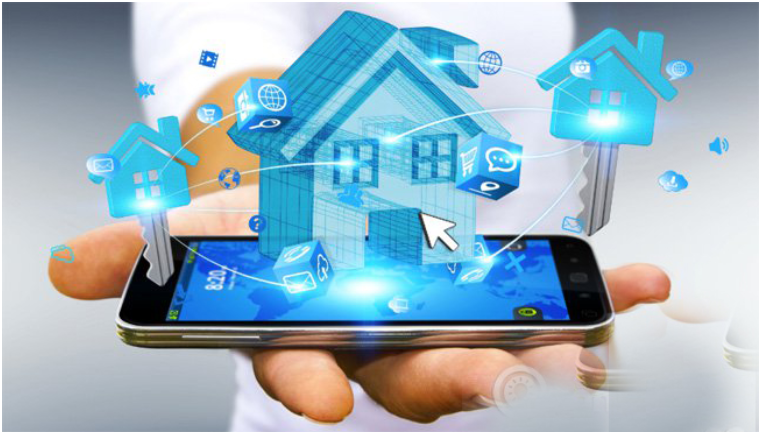
\includegraphics[scale=0.6]{image1/marthome.png}
    \end{center}
    \caption{Smarthome.}
    \label{refhinh1}
    \end{figure}
\end{center}
    \item Các thiết bị đeo thông minh\\
    Hiện nay ở nhiều nước đã xuất hiện các thiết bị đeo trên người với những tính năng vô cùng thông minh như: tai nghe, các loại kính, ba lô, vòng tay siêu thông minh,… Những thiết bị này dần bùng nổ tại các thị trường trên toàn thế giới. Google và Samsung là những công ty lớn có những khoản đầu tư khổng lồ cho việc tạo ra các thiết bị như vậy. Các thiết bị đeo được cài đặt cảm biến và các phần mềm thu thập dữ liệu, thông tin người dùng. Các thiết bị này bao gồm các yêu cầu về thể chất, sức khỏe và có tính giải trí cao. Điều kiện tiên quyết cho các thiết kế này là công suất cực thấp và kích thước nhỏ gọn, có tính thẩm mỹ cao.
\newpage
 \begin{center}
    \begin{figure}[htp]
    \begin{center}
     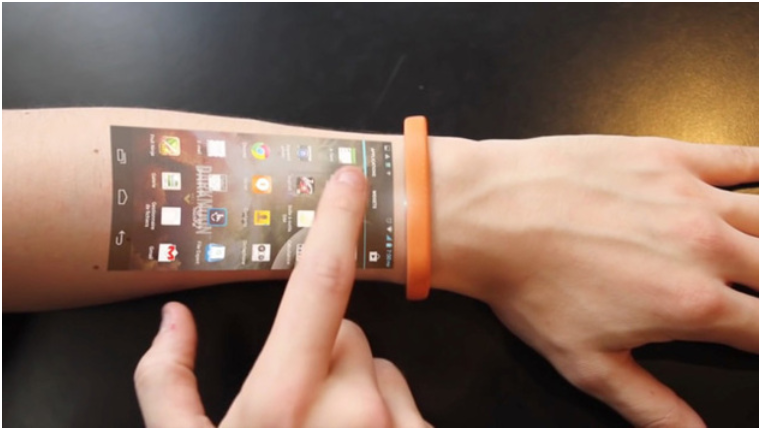
\includegraphics[scale=0.6]{image1/thietbi.png}
    \end{center}
    \caption{Thiết bị đeo tay thông minh.}
    \label{refhinh1}
    \end{figure}
\end{center} 
    \item Những chiếc ô tô được kết nối
 \begin{center}
    \begin{figure}[htp]
    \begin{center}
     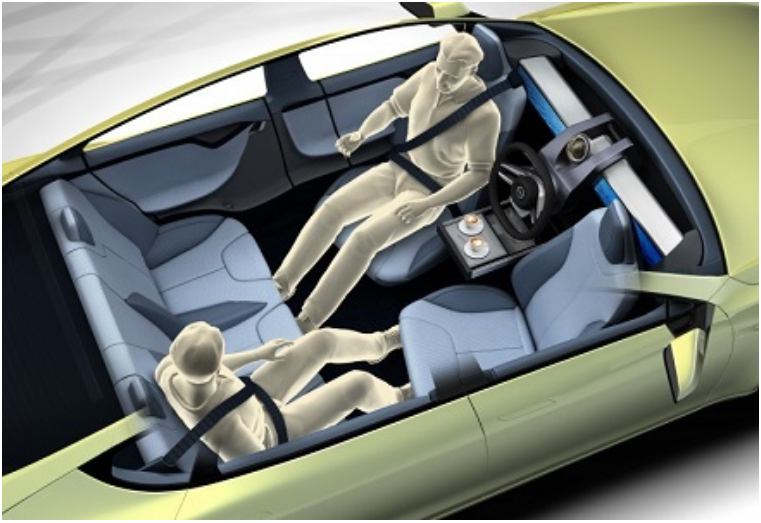
\includegraphics[scale=0.5]{image1/oto.png}
    \end{center}
    \caption{Ô tô thông minh.}
    \label{refhinh1}
    \end{figure}
\end{center} 
    Các nhà sản xuất ô tô đã bước qua giai đoạn tập trung vào việc tối ưu hóa các chức năng nội bộ của một chiếc xe. Giờ đây họ quan tâm đến việc tối ưu hóa sự hài lòng của người sử dụng với việc nâng cao trải nghiệm trong xe hơi.

    Một chiếc xe được kết nối là chiếc xe có khả năng tối ưu hóa hoạt động, bảo trì cũng như sự thoải mái của khách hàng khi sử dụng. Các thương hiệu lớn như BMW, Tesla, … đang nỗ lực cho cuộc cách mạng tiếp theo của ngành sản xuất ô tô.
    
    \item Internet công nghiệp
 \begin{center}
    \begin{figure}[htp]
    \begin{center}
     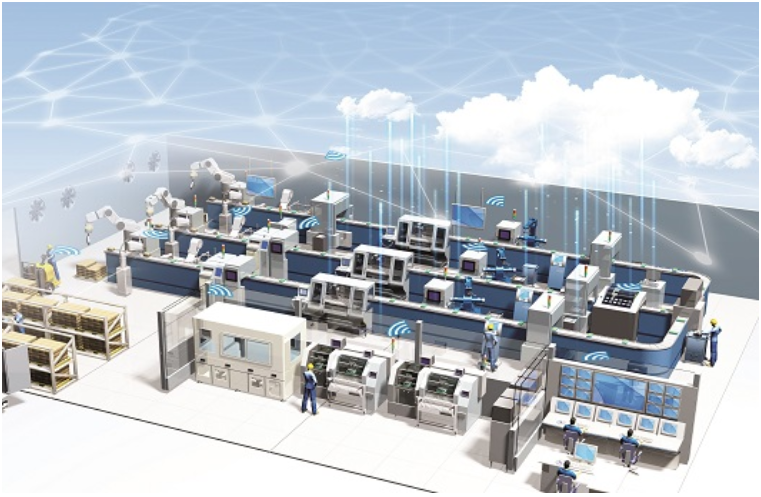
\includegraphics[scale=0.6]{image1/congnghiep.png}
    \end{center}
    \caption{Internet công nghiệp.}
    \label{refhinh1}
    \end{figure}
\end{center} 
    Industrial Internet là tiếng vang mới trong ngành công nghiệp, được gọi tắt là IIoT (Industrial Internet of Thing). IIoT hỗ trợ kĩ thuật công nghiệp với các cảm biến, phần mềm lớn để tạo ra những cỗ máy vô cùng thông minh. Máy móc sẽ có tính chính xác và nhất quán hơn con người trong giao tiếp thông qua dữ liệu. Từ những dữ liệu thu thập được giúp các công ty, nhà quản lí giải quyết các vấn đề sớm hơn, đạt hiệu quả cao hơn.

    IIoT có tiềm năng lớn về kiểm soát chất lượng và tính bền vững. Những ứng dụng trao đổi thông tin giữa nhà cung cấp, nhà phân phối và nhà bán lẻ về thông tin hàng hóa, hàng tồn kho sẽ làm tăng hiệu quả chuỗi cung ứng.
    
    \item Smart city
    Thành phố thông minh là một ứng dụng của IoT tạo được sự tò mò của đông dảo người dân. Giám sát thông minh, vận chuyển tự động, hệ thống quản lý năng lượng thông minh hơn, phân phối nước, an ninh đô thị và giám sát môi trường tất cả là ví dụ về internet của các ứng dụng cho thành phố thông minh. IoT giúp giải quyết các vấn đề gặp phải tại các thành phố lớn đó là ô nhiễm môi trường, tắc nghẽn giao thông và thiếu năng lượng. Một ví dụ có thể kể đến của các thiết bị được sử dụng truyền thông di động như: thùng rác thông minh, chúng sẽ gửi cảnh báo đến bộ phận vệ sinh môi trường khi cần dọn sạch.

    Bằng cách cài đặt ứng dụng và dùng các thiết bị thông minh chúng ta hoàn toàn có thể dễ dàng tìm thấy các cây xăng, siêu thị, quán ăn hay thậm chí là những bãi gửi xe miễn phí. Ngoài ra hệ thống điện cũng được bảo vệ bởi các cảm biến sẽ giúp phát hiện nhanh chóng các vấn đề gây nhiễu, trục trặc, hay các vấn đề về lắp đặt.
    
\begin{center}
    \begin{figure}[htp]
    \begin{center}
     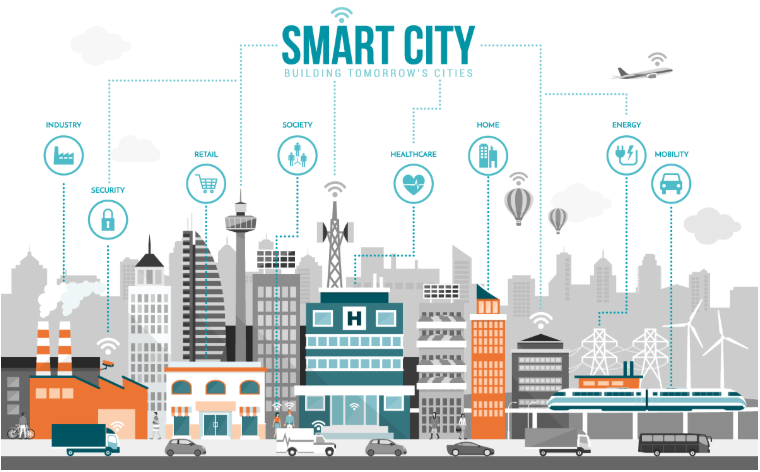
\includegraphics[scale=0.6]{image1/city.png}
    \end{center}
    \caption{Smart city.}
    \label{refhinh1}
    \end{figure}
\end{center} 
    \item IoT trong nông nghiệp
    Với sự gia tăng liên tục của dân số đồng nghĩa với việc nhu cầu sử dụng lương thực tăng lên nhiều lần. Nông dân có thể áp dụng các kỹ thuật mới, công nghệ tiên tiến để tăng sản lượng sản xuất nông nghiệp. Nông nghiệp thông minh có thể nói là lĩnh vực phát triển nhanh nhất với IoT.

    Những thông tin người nông dân thu được giúp họ có những quyết định đầu tư sáng suốt tránh tình trạng “được mùa mất giá, được giá mất mùa” như hiện nay. Cảm biến độ ẩm, chất dinh dưỡng của đất, mức độ hấp thụ nước góp phần quan trọng vào việc kiểm soát sự tăng trưởng của cây trồng giúp người gieo trồng có thể xác định, tùy chỉnh lượng phân bón cần thiết.
\begin{center}
    \begin{figure}[htp]
    \begin{center}
     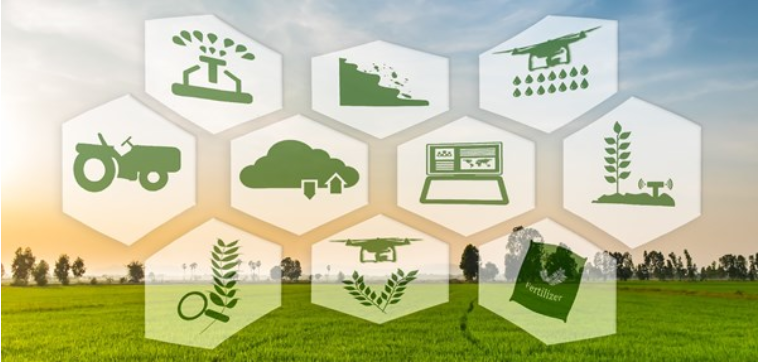
\includegraphics[scale=0.6]{image1/nongnghiep.png}
    \end{center}
    \caption{IoT trong nông nghiệp.}
    \label{refhinh1}
    \end{figure}
\end{center} 

    \item Bán lẻ thông minh
    IoT tạo nên một sự kết nối mật thiết giữa nhà bán lẻ với khách hàng giúp nâng cao trải nghiệm của khách hàng khi đến với cửa hàng. Tiềm năng phát triển IoT trong lĩnh vực bán lẻ là vô cùng lớn.

    Smart phone là thiết bị phổ biến nhất được sử dụng để các nhà bán lẻ duy trì kết nối với khách hàng của mình khi khách hàng đến với cửa hàng hay thậm chí ngay cả khi họ ra khỏi cửa hàng. Tương tác qua điện thoại và việc sử dụng các công nghệ giúp cho các nhà bán lẻ phục vụ khách hàng tốt hơn, thay đổi cách bài trí cửa hàng cho phù hợp với nhu cầu tiêu dùng.
\newpage 
\begin{center}
    \begin{figure}[htp]
    \begin{center}
     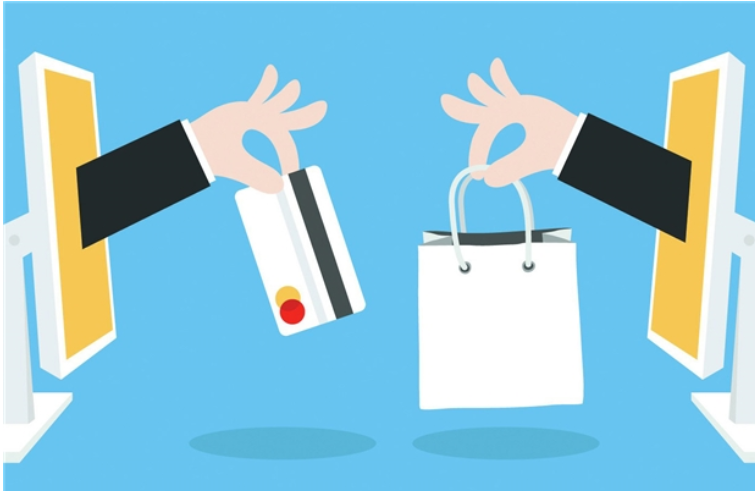
\includegraphics[scale=0.6]{image1/banle.png}
    \end{center}
    \caption{Bán lẻ thông minh.}
    \label{refhinh1}
    \end{figure}
\end{center} 
    \item Năng lượng
\begin{center}
    \begin{figure}[htp]
    \begin{center}
     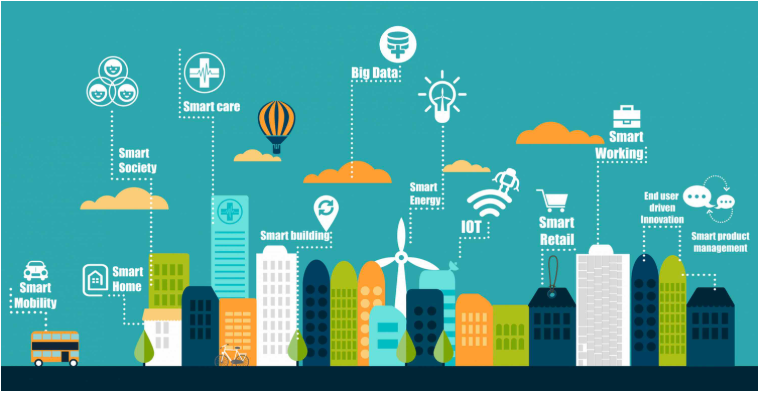
\includegraphics[scale=0.6]{image1/nangluong.png}
    \end{center}
    \caption{Năng lượng.}
    \label{refhinh1}
    \end{figure}
\end{center} 
    Mạng lưới điện trong vài năm tới sẽ trở nên thông minh và đáng tin cậy hơn. Khái niệm lưới điện thông minh đang trở nên phổ biến trên toàn thế giới.

    Dữ liệu được thu thập một cách tự động để phân tích hành vi tiêu dùng điện của người dùng và nhà cung cấp để góp phần nâng cao hiệu quả sử dụng điện. Lưới điện thông minh giúp phát hiện nguồn ngắt điện thông minh ở cấp độ các hộ gia đình.
    
    \item Sức khỏe
\begin{center}
    \begin{figure}[htp]
    \begin{center}
     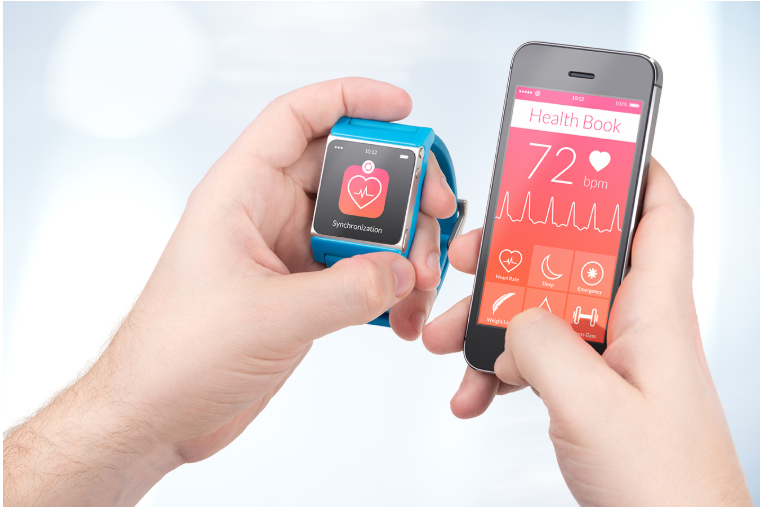
\includegraphics[scale=0.6]{image1/suckhoe.png}
    \end{center}
    \caption{Sức khỏe.}
    \label{refhinh1}
    \end{figure}
\end{center} 
    Đây có thể nói là một lĩnh vực chưa được khai phá hết của Internet of Things bởi những ứng dụng không ngờ mà nó mang lại. Một hệ thống chăm sóc sức khỏe được kết nối cùng các thiết bị y tế thông minh mang lại tiềm năng to lớn cho các công ty đầu tư sản xuất. IoT trong chăm sóc sức khỏe giúp mọi người có cuộc sống khỏe mạnh hơn bằng việc đeo các thiết bị kết nối. Các dữ liệu thu thập được giúp phân tích sức khỏe của người dùng thiết bị kết nối và nhà cung cấp, sản xuất sẽ có được những thiết kế để chống lại bệnh tật.
    
    \item IoT và chăn nuôi gia cầm, sản xuất nông trại.
    Kiểm soát các khâu trong quy trình chăn nuôi giúp tiết kiệm thời gian và chi phí. Sử dụng các công cụ IoT để thu thập dữ liệu về sức khỏe của gia súc, các chủ trang trại có thể biết sớm về bệnh tật của động vật giúp ngăn ngừa số lượng lớn các gia súc bị bệnh bởi virus lây lan. Với những dữ liệu thu thập được cũng giúp chủ trang trại tăng nhanh được sản lượng gia súc, gia cầm.

\begin{center}
    \begin{figure}[htp]
    \begin{center}
     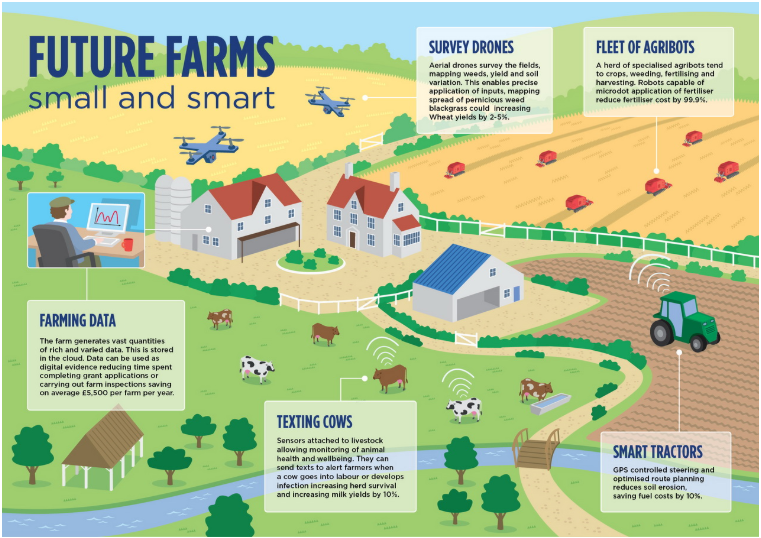
\includegraphics[scale=0.6]{image1/nongtrai.png}
    \end{center}
    \caption{IoT và chăn nuôi gia cầm, sản xuất nông trại.}
    \label{refhinh1}
    \end{figure}
\end{center} 
\end{enumerate}

Trong tương lai những gì IoT mang lại sẽ vượt xa những ứng dụng kể trên. IoT sẽ mang lại sự thay đổi tầm vĩ mô trong cách con người sống và làm việc\cite{tl13}.
\section{Các thách thức hiện tại của mạng IoTs}
Internet of Things - IoT có thể xem là đại diện của mọi thiết bị thông minh nhưng xu hướng này còn gặp nhiều khó khăn trong việc triển khai một cách toàn diện. IoT theo định nghĩa hiểu đơn giản là các bộ cảm biến có thể giao tiếp với Internet mà không cần có sự can thiệp của con người. Định nghĩa đó bao gồm cả các thiết bị đeo và điện thoại thông minh, hay các thiết bị có thể tự động giao tiếp nếu được cấp phép. IoT cũng bao gồm các thiết bị thông minh dành cho xe hơi, nhà ở và kể cả một thành phố hay thiết bị y tế hoặc công cụ trong các ngành công nghiệp. Những lợi ích và tiềm năng phát triển của IoT ở khắp mọi nơi, ở đâu có kết nối đều có khả năng xuất hiện các thiết bị với định danh của riêng mình, mang đến giá trị thông qua truyền tải, trao đổi thông tin, dữ liệu. Có thể thuật ngữ này sẽ biến mất khi IoT trở thành một chuẩn mực, và có thể được thay thế bằng một cái tên gọi khác nhằm ám chỉ những thiết bị không thể giao tiếp. Nhưng một số thách thức có thể làm trì hoãn tương lai của IoT và sau đây là những trở ngại đáng chú ý.\\
\begin{itemize}
\item \textbf{An ninh và bảo mật dữ liệu}: IoT đã trở thành một mốt quan tâm đáng lo ngại về an ninh, nó đã thu hút sự chú ý của các công ty công nghệ nổi tiếng và các cơ quan chính phủ trên toàn thế giới. Việc hack vào các thiết bị IoT như màn hình theo dõi em bé, tủ lạnh thông minh, máy bơm nước, điều hòa nhiệt độ, camera hay thậm chí là radio trong ô tô đang trở thành mối lo ngại về an ninh do sự phát triển của IoT gây ra. Vì vâỵ, các thiết bị mới được thêm vào mạng sẽ là yếu tố để các hacker có thể tấn công và xâm nhập dữ liệu trái phép vì số lượng lỗ hổng bảo mật là khá đáng kể.
Mọi vấn đề bảo mật chỉ tốt khi chúng ta có thể chỉ ra các điểm yếu của thiết bị, và đối với một thế giới kết nối như hiện nay thì điều đó có rất nhiều.\\

Điều này giải thích lý do tại sao Samsung đã dành nỗ lực đáng kể vào nền tảng ARTIK dành cho IoT trong thời gian gần đây. ARTIK có 3 mẫu module chứa tất cả các thành phần – bộ cảm biến, vi xử lý, bộ nhớ tích hợp, và kèm theo đó là khả năng kết nối không dây cần thiết cho các nhà sản xuất để tạo ra thiết bị thông minh. Tất cả các module ARTIK đều được hãng trang bị một khoá an toàn nhằm giúp các nhà phát triển mã hoá dữ liệu tốt hơn so với phần mềm mã hoá mặc định.\\

Đối với các thiết bị cá nhân có khả năng kết nối Internet thì vấn đề an ninh và sự riêng tư là những mối quan tâm hàng đầu. Đây có lẽ là những sản phẩm điển hình để được trang bị hệ thống mã hóa, nhưng vấn đề an ninh và sự riêng tư lại có đặc thù riêng khác nhau. An ninh bảo mật thường gằn liền với công nghệ còn sự riêng tư thì thương liên quan đến con người và tính pháp lý. Các nhà sản xuất thiết bị IoT cần phải hiểu rằng an ninh và sự riêng tư không thể đồng nhất hoặc áp dụng chung mọi quy tắc. Khả năng giao tiếp tự động của thiết bị IoT làm cho việc đảm bảo sự riêng tư khó khăn hơn bởi các mô hình sản phẩm được khuyến khích sử dụng trước khi có sự đồng thuận của người dùng ở những thời điểm khác nhau.\\

\item \textbf{Tiêu chuẩn chung}: Việc thiếu các tiêu chuẩn, đặc biệt là trường hợp sử dụng nhiều giao thức kết nối như hiện nay, là một cản trở cho IoT phát triển. Nhiều giao thức kết nối đặc biệt đang nổi lên với mức tiêu thụ năng lượng thấp như LTE Cat.0, 802.11ah, Sigfox hay OnRamp. Công nghệ bộ xử lý hiện cũng chưa thực sự hào hứng với thị trường IoT khi chuẩn giao thức không thực sự rõ ràng.\\

Các hãng công nghệ như LG, Panasonic, Sharp, Silicon Image, TP-Link, HTC, Qualcomm và hơn 100 thành viên khác đã thành lập nên liên minh AllSeen, dẫn đầu là Hiệp hội Linux. Tiêu chí của liên minh này là xóa bỏ những rào cản cũng như thúc đẩy sự sáng tạo trong việc phát triển Internet of Things. Nhóm này đã xây dựng nên nền tảng nguồn mở AllJoyn cho phép các sản phẩm IoT có thể giao tiếp với nhau thông qua nhiều dạng kết nối từ Wi-Fi, Ethernet, và cả đường dây điện. AllJoyn có thể tương thích với mọi hệ điều hành hiện nay và cũng không bắt buộc các thiết bị phải kết nối vào Internet bởi chúng có thể liên lạc ở cấp độ ngang hàng\\

Open Internet Consortium (OIC): Đây được xem là đối thủ của AllSeen Alliance, tổ chức OIC được các ông lớn công nghệ gồm Intel, Broadcom, Dell và Samsung chống lưng nhằm phát triển các tiêu chuẩn và chứng nhận cho các thiết bị Internet of Things. Các tiêu chuẩn này cũng xoay quanh khả năng giao tiếp và chứng thực thiết bị dựa trên các giao thức kết nối khác nhau gồm Wi-Fi, Bluetooth và cả NFC.\\

Thread Group: Tổ chức phi lợi nhuận này được thành lập bởi Nest Labs (thuộc Google), Samsung, ARM, Freescale, Silicon Labs... Thread Group tạo ra một giao thức mạng không dây dựa trên IP, cho phép các thiết bị phần cứng trong nhà kết nối với đám mây. Mục tiêu mà Thread Group còn nhắm đến việc giảm mức tiêu thụ năng lượng của thiết bị và đảm bảo tính an toàn bảo mật kết nối với IPv6. Tổ chức này dường như chỉ tập trung vào nền tảng hạ tầng hoạt động của IoT chứ không can thiệp quá nhiều vào phần cứng. Điều này cũng giúp dễ dàng tương thích với các tiêu chuẩn khác như AllSeen hay OIC.\\

Industrial Internet Consortium (IIC): Đây là tổ chức thứ 2 mà Intel tham gia vào nhằm phát triển IoT, ngoài ra General Electric, Cisco Systems, IBM và nhà mạng AT\&T là những thành viên thành viên tích cực nhất. Tuy nhiên, IIC tập trung vào mảng thiết bị IoT dùng cho doanh nghiệp và đảm bảo mọi thứ cùng hoạt động tốt ở mọi phân khúc thị trường. Ngoài ra, IIC giúp cải tiến các hệ thống máy móc lỗi thời có thể tham gia vào hệ thống IoT.\\

IEEE P2413: Viện kĩ thuật điện điện tử (IEEE) là một trong những tổ chức chính quy có nhiệm vụ đặt ra các tiêu chuẩn quan trọng trong thế giới công nghệ. Nhưng trong xu hướng IoT thì IEEE bị các công ty công nghệ cho rằng quá chậm chạp trong việc thiết lập tiêu chuẩn. IEEE quy tụ 23 nhà sản xuất có liên quan và cùng nghiên cứu tạo nên bộ chuẩn chung cho thiết bị.\\

\item \textbf{ Kết nối}: Kết nối rất nhiều thiết bị sẽ là một trong những thách thức lớn nhất của tương lai IoT, và sẽ phải tái cấu trúc các mô hình truyền thống hiện tại và công nghệ kết nối. Hiện tại, chúng ta đang dựa và mô hình tập trung, server-client để xác thực, ủy quyền các nút khác nhau trong một mạng.\\

Mô hình này là đủ cho hệ sinh thái IoT hiện tại, khi hàng chục, hàng trăm, hàng nghìn thiết bị kết nối. Nhưng khi IoT phát triển, hàng tỷ và hàng trăm tỷ thiết bị kết nối, hệ thống tập trung hiện tại sẽ bị thắt cổ chai. Các hệ thống lớn để đáp ứng số lượng lớn thiết bị này sẽ yêu cầu sự đầu tư khổng lồ vào các máy chủ đám mây để có thể xử lý lượng trao đổi thông tin khổng lồ.\\

IDC và EMC ước tính rằng tới năm 2020, sẽ có 44 nghìn tỉ gigabyte dữ liệu trên thế giới và 10 trong số đó là đến từ các thiết bị IoT. Mức này tương đương với 4.4 nghìn tỉ gigabyte, đồng thời cũng tương đương với mức dung lượng tất cả dữ liệu trên thế giới ước tính vào năm 2013. Nói cách khác, sức chứa của tất cả các trung tâm dữ liệu trực tuyến trong năm 2013 chỉ đủ để lưu trữ dữ liệu IoT trong năm 2020. Điều này sẽ có ảnh hưởng lớn tới cách các trung tâm dữ liệu làm việc để chúng có thể chịu được lượng dữ liệu lưu trữ trên đám mây khi các dữ liệu này được tạo ra và trao đổi.\\

\begin{figure}[htp]
\begin{center}
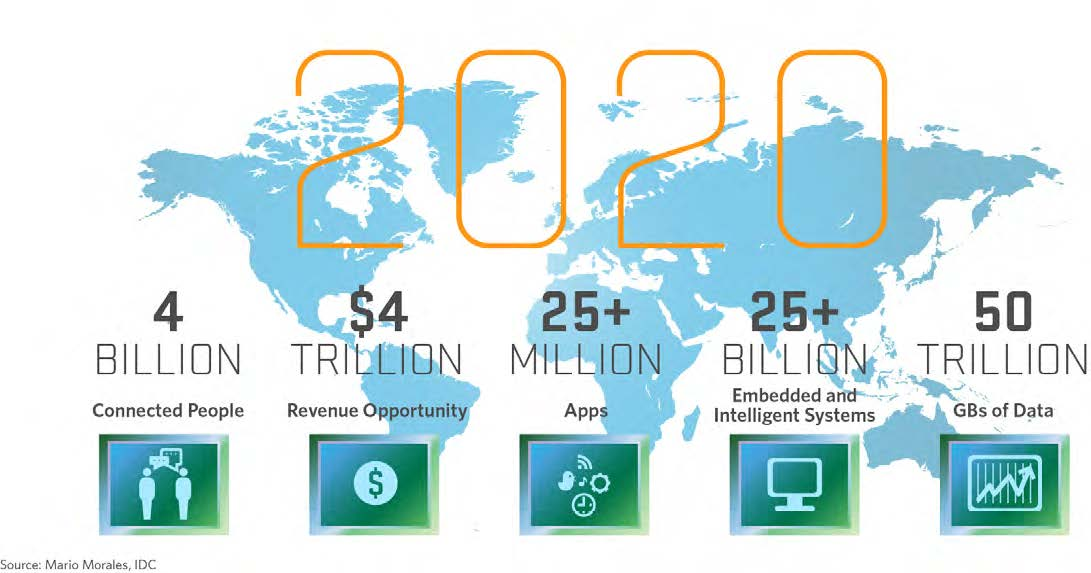
\includegraphics[scale=1]{image1/IoT.jpg}
\end{center}
\caption{Dự đoán IoT đến năm 2020}
\label{IoT2020}
\end{figure}
\newpage
Còn quan trọng hơn cả là yêu cầu kết nối để giúp tất cả các thiết bị này giao tiếp với nhau, để có thể gửi dữ liệu đến và đi khỏi kho lưu trữ dữ liệu trực tuyến. Giao thức IPv6 được tạo đã phần nào nghĩ tới tương lai này khi nó hỗ trợ $2^{128}$ địa chỉ, so với chỉ $2^{32}$ địa chỉ của giao thức IPv4. Lưu lượng dữ liệu trên 1 thiết bị cá nhân có thể không quá nhiều. Bluetooth cũng có thể đủ dùng với nhiều mạng cảm biến đòi hỏi mức năng lượng thấp, và rất nhiều trong số này cũng được tải lên rải rác chứ không stream mọi thông tin cùng 1 lúc.\\

Thế nhưng, tổng hợp hàng tỉ thiết bị trực tuyến vào năm 2020 và tất cả lượng băng thông sẽ là rất lớn. Quản lý dung lượng kết nối mạng một cách cẩn trọng sẽ là việc vô cùng thiết yếu.
\end{itemize}

\section{Giới thiệu đề luận văn}
Với sự phát triển của Internet of Things (IoTs), rất nhiều ứng dụng tiện ích đã được hiện thực. Tuy nhiên, các ứng dụng hiện tại đều tập trung vào việc gửi dữ liệu trực tiếp từ node cảm biến về node trung tâm. Điều này làm cản trở việc triển khai ứng dụng trên diện rộng, khi tầm bao phủ của ứng dụng lớn hơn phạm vi gửi dữ liệu không dây. Do đó, việc phát triển một nền tảng cho phép gửi dữ liệu qua nốt trung gian (multi-hop) sẽ mở ra nhiều cơ hội cho việc triển khai ứng dụng. Bên cạnh đó, node trung tâm cũng cần dựa trên một hệ điều hành, thay vì chủ yếu là nền tảng vi điều khiển như hiện tại, để có thể hỗ trợ nhiều xử lý đa dạng và phức tạp (ví dụ: kết nối 3G, cập nhật firmware từ xa) cũng như nâng cao độ ổn định của hệ thống.\\
\subsection{Mục tiêu của luận văn}
Xây dựng hệ thống thu thập dữ liệu trên nền tảng mạng cảm biến không dây multi-hop và hệ điều hành nhúng phục vụ cho ứng dụng Internet of Things.
\subsection{Mục tiêu cụ thể của giai đoạn thực tập}
Tìm hiểu các chuẩn giao tiếp không dây hiện có, lựa chọn tiêu chuẩn giao tiếp phù hợp dựa vào các tiêu chí: tầm xa, năng lượng, độ ổn định (tỉ lệ lỗi thấp).
\newline
Tìm hiểu các hệ điều hành nhúng đang được hỗ trợ phổ biến cho các mạng cảm biến IoTs (ví dụ: Android things, Windows things,…). Lựa chọn hệ điều hành phù hợp cho đề tài.
\subsection{Các ứng dụng tiềm năng cho kết quả của luận văn}
Xây dựng một ứng dụng giám sát trên phạm vi rộng (ví dụ môi trường nước hoặc môi trường không khí) để kiểm tra tính đúng đắn của đề tài.




